\chapter{Multi-Hypotheses Kalman Filter Localization\label{cha:chapter5}}
While the Kalman filter can only deal with uni-modal probability distribution, it does not suffice to handle the ambiguous landmarks that occur in robot's observation, which requires a multi-modal distribution. Therefore, a multi-hypotheses Kalman filter is adapted to handle the ambiguous situations by describing the robot position in the field by a Gaussian sum distribution.
The problem of multi-hypotheses Kalman filter lies mainly in the domain of when and where to add new hypothesises into the Gaussian sum distribution, as well as when to prune or merge certain hypotheses to restrain the number of hypotheses within a limit, so it does not consume too much of the computation resources.


\section{Hypothesis Model Weighting}
As illustrated in \autoref{sub:mmkalman}, each normal probability distribution from the Gaussian sum distribution is represented as \autoref{eq:mmkalman}. In addition to uni-modal Gaussian distribution, the weight $\alpha_i$ has to be determined for each Gaussian distribution model $i$ in the Gaussian sum distribution. The weight, at the same time, illustrates the quality of the state hypothesis. Possible update method like \autoref{eq:weightupdate} has been proposed in \cite{alspach1972nonlinear}. However, this update method is only suitable for landmarks with known correspondence. If the correspondence is unknown or ambiguous, like in our case, the ``T'' junctions, the expected observation $z\widehat{}_i$ can not be determined. 

In this thesis, a voting buffer is used to measure the weight of each model. The voting buffer is constructed by a \gls{FIFO} circular buffer of size $60$. The basic idea is to vote $1$ to the buffer when the observed landmark is matched, and $0$ when not matched. The matching of landmark correspondence is using the nearest neighbor algorithm with threshold discussed in \autoref{subsub:landmarkco}. 
The advantage of using a circular buffer is that, after $60$ observed landmarks, regardless matched or not, the old voting in the buffer will be flushed and will not be counted. In other words, it tries to approximate the current robot state by keeping the memory of the most recent history. The model weight is determined by the average value of the voting buffer. Therefore, the more matches with landmarks the Kalman model makes, the higher weight it will have. 

Unlike the implementation of particle filter that the total number of particles are fixed, in multi-hypothesis Kalman filters, the number of hypothesis model is dynamic. The adjustment made here is that the weights of all the Gaussian models do not add up to 1, instead they each behave independently. So the weights of the existing hypothesis models will not be affected by the newly generated ones.

As discussed in subsection \ref{subsub:landmarkco}, some landmarks are unique landmarks, \ie{} center circle, and some are ambiguous landmarks, \ie{} junctions and lines. To depict the quality of the robot localization state, the vote should depend only on the globally unique landmarks instead of ambiguous landmarks. Assume a scenario, where the robot is not moving and constantly observing a ``T'' junction, and the ``T'' junction is perfectly matched with its nearest neighbor in the field. In this case, the state of the robot position is local optimal. The weight of the model will keep increasing and reach 1, but this weight is not truly describing the quality of localization state in global. 

To better express the localization state globally, in the localization algorithm, landmarks are classified differently to update the weight. In observation, center circle with/without orientation and penalty area are treated as unique landmarks, they can directly vote 1 to the voting buffer when the threshold requirement in the nearest neighbor algorithm is satisfied, or vice versa. 

On the other hand, ``L'', ``T'', ``X''junctions are classified as non-unique landmarks, the voting buffer can be voted by 1, only when at least two junctions are matched, and in addition they must each belong to different junctions in the field. The junctions under consideration do not distinguish ``L'', ``T'' or ``X'', and they can come from different observation frames, as long as there is no failure match (beyond threshold) in between. By using the combination of the different observations of junctions, we assume it represents a global unique landmark, thus helping to overcome the local optimal problem. While the requirement of voting positive using junctions is strict, the condition of voting 0 is the same as the unique landmarks, \ie{} when a failure match happens for the junction, a 0 will be voted to the buffer.  

For the observed line landmarks, they are currently not contributing to the voting buffer. To utilize the lines, certain feature structures need to be extracted from them, in order to use the same strategy above to update the voting buffer. However, the extraction of other features out of the lines is not an easy task, further work may be required in this regard in the future. 
%summing up the values in the voting buffer and calculate the average.


\section{Landmark Based Resampling}\label{sec:resample}

Similar to the augmented particle filter's \cite{thrun2005probabilistic} sensor reseting step to recover the situation of robot getting kidnapped, multi-hypotheses Kalman filter uses sensor reseting based on landmarks to recover from position tracking failure. Assume uni-modal Kalman filter for position tracking, the filter can lose track of the robot's position when the robot is hit by another robot which results in an error in robot's orientation; or the robot is kidnapped by a referee during manual replacement, etc. Augmented particle filter initiates the sensor resetting step to generate random particles when the fluctuation of the weights from the particles is high, multi-hypotheses Kalman filter designed in this thesis will start resampling when an observed landmark fails to match the one on the field. Here, a correspondence match failure is regarded as a signal for potential loss of position tracking. 

The resampling is achieved by calculating all the possible poses of the robot with respect to the observation of the landmark. The landmarks which can trigger resampling are the landmarks with orientation, \ie{} center circle with center line and all kinds of junctions. The landmarks without orientation like lines, center circle without center line and penalty area can generate infinite possible robot positions, therefore currently they are not used for resampling. The problem of calculating the possible poses can be formulated as follows:

Given an observed landmark $l_R = (x_R, y_R, \theta_{R})$ in robot frame, and assume its correspondent landmark $l_G = (x_G, y_G, \theta_{G})$ in physical world frame, the corresponding robot pose in physical world frame is what is needed to be calculated. The calculation concerns mainly with the coordinate frame transformation which can be described by homogeneous transform matrix. 

A homogeneous transform matrix in our context is a $3 \times 3$ matrix. It is structured by a $2 \times 2$ rotation matrix $R_B^A$ and a $2 \times 1$ translation matrix  $P_B^A$ denoted in \autoref{eq:homomat}.
\begin{equation}
\label{eq:homomat}
T_B^A =
\begin{bmatrix}
R_B^A & P_B^A \\
\bf{0}   & 1 
\end{bmatrix}
\end{equation}

The sub and super-script in $R_B^A$ indicate that it is the rotation of frame $B$ relative to frame $A$. Translation matrix  $P_B^A$ denotes the translation of the origin of frame $B$ in frame $A$.
In the following equations, we represent the robot pose in physical world frame in the form of  homogeneous transform matrix as $T_R^G$, landmark in robot frame as  $T_L^R$, landmark in physical world frame as $T_L^G$.
According to \textit{Composition Rule for Homogeneous Transformations}, the transformation between $T_R^G$, $T_L^R$ and $T_L^G$ can be described in \autoref{eq:trans}.
\begin{equation}
\label{eq:trans}
T_R^G \cdot T_L^R=T_L^G
\end{equation}

To obtain $T_R^G$, we multiply $(T_L^R)^{-1}$ from the right for both side of the equation, then obtain \autoref{eq:reverseTrans}.

\begin{equation}
\label{eq:reverseTrans}
	T_R^G=T_L^G\cdot (T_L^R)^{-1} 
\end{equation}

Substituting the homogeneous transform matrix using \autoref{eq:homomat}, and calculating the inverse of matrix, results in the following:
\begin{equation}
\label{eq:reverseTrans2}
	T_R^G=
\begin{bmatrix}
R_L^G & P_L^G \\
\bf{0}   & 1 
\end{bmatrix} \cdot
\begin{bmatrix}
  (R_L^R)^\top & -(R_L^R)^{\top} P_L^R \\
\bf{0}   & 1 
\end{bmatrix}
\end{equation}


\begin{equation}
\label{eq:reverseTrans3}
	T_R^G=
\begin{bmatrix}
  R_L^G(R_L^R)^\top & -R_L^G(R_L^R)^{\top} P_L^R +  P_L^G\\
\bf{0}   & 1 
\end{bmatrix}
\end{equation}

By using the rotation matrix representation stated in \autoref{eq:rot}, the rotation matrix and translation matrix in $T_R^G$ is calculated in  \autoref{eq:reverseTrans4} and \autoref{eq:reverseTrans5}.
\begin{equation}
\label{eq:reverseTrans4}
	R_R^G=
	R_L^G(R_L^R)^\top =
  \Omega(\theta_{G} - \theta_{L}) 
\end{equation}

\begin{equation}
\label{eq:reverseTrans5}
	P_R^G=
	-R_R^G P_L^R +  P_L^G=
   -\Omega(\theta_{G} - \theta_{L}) \cdot
\begin{bmatrix}
  x_R\\
  y_R
\end{bmatrix}
+
\begin{bmatrix}
  x_G\\
  y_G
\end{bmatrix}
\end{equation}

Therefore, given the correspondence of $l_R$ and $l_G$,  the robot x-y position is $P_R^G$ and orientation is $\theta_{G} - \theta_{L}$. The number of possible robot poses generated depends on the occurrence of the landmarks in the field. For example, a mismatch of a ``T'' junction would trigger resampling which would generate 14 possible robot poses. The weight for the newly generated hypothesis model is 1 divided by the number of occurrences of the landmarks in the field. So, in the case for resampling by ``T'' junction, the weight for the new hypothesis model is $1/14 = 0.0714$. However, the model resampled by center circle is an execution as only one model will be generated. The weight of this model will be directly proportional to the detection confidence of the center circle.

\subsection{``L'' Junction Look Up Table}
\label{sub:Junction Look Up Table}
A special case worths discussing is the observation of the ``L'' junctions, as there are 36 occurrences of ``L'' junctions in the field, a match failure can resample as much as 36 possible robot positions, the weight for the newly generated hypothesis model will be $1/36=0.027$ which is extremely low. Such low weight model can be easily pruned in the pruning step which we will discuss in \autoref{sec:pruning}. However, due to the large number of occurrences of ``L'' junctions, the possibility of observing more than one ``L'' junctions at the same frame is also high. When more than one ``L'' junctions are observed in one frame, the number of possible positions can also be reduced. Given the ``L'' junctions observed, the implementation to generate possible positions due to multiple ``L'' junctions is described in the following steps:

\begin{enumerate}
  \item Take one observed ``L'' junction, use \autoref{eq:reverseTrans4} and \autoref{eq:reverseTrans5} to generate 36 possible robot positions based on all the ``L'' junctions in the field. 
  \item Take another observed ``L'' junction, at each robot position generated in Step 1, project the ``L'' junction to the physical world frame.
  \item Check if at the place where the observed ``L'' junction is projected, there exists an  ``L'' junction in the field. If so, this generated robot position is valid, otherwise it is an invalid position.
  \item If there are remaining ``L'' junctions in observation, steps from Step 2 are repeated. Otherwise, the possible robot positions which are valid are returned.
\end{enumerate}

To speed up the computation, Step 3 above is implemented using a pre-computed look up table. Given a pose $(x_l, y_l, \theta_l)$ of the ``L'' junction in physical world frame,  the look up table will return boolean value, \ie{} true or false, depending on whether in the vicinity of pose $(x_l, y_l, \theta_l)$, there exists an ``L'' junction. Although it is a 3-dimensional look up table, the resolution can be configured coarse, it will not consume too much memory. In return, the checking of 36 ``L'' junctions in physical world frame can be done together at once. A visualization example of the look up table is illustrated in \autoref{fig:lcornerLUT}. Since it is a 3-dimensional look up table, \autoref{fig:lcornerLUT} only shows the look up table when the angle dimension is at \SI{90}{\degree}. It means, if given an ``L'' junction in physical world frame with angle being \SI{90}{\degree}, only the ``L'' junctions which fall into the bright area is valid. %The correctness can be verified by checking in correspond with \autoref{fig:ljunctions}.

\begin{figure}
\begin{center}
	\includegraphics[width=0.8\textwidth]{fieldwithLcornerslut.png}
\end{center}
\caption[``L'' junction look up table]{``L'' junction look up table with angle dimension at \SI{90}{\degree}. Bright parts indicate true, dark parts indicate false}
\label{fig:lcornerLUT}
\end{figure}

To further reduce the number of sampled positions by ``L'' junction, we retain only the positions which are close enough to the last robot position. With the filtering of the positions generated by ``L'' junctions, the weight of the sampled position is set to be the same as the ones generated by ``T'' junctions.

\section{Best Hypothesis Model and Confidence}\label{sec:robotpose}
In multi-hypothesis Kalman filter, there are multiple hypothesis models to form the possibility distribution. From the robot position probability distribution, one position $(x_{r}(t), y_{r}(t), \theta_{r}(t))$
has to be determined as the end result of localization algorithm. In the algorithm designed, the position is chosen to be the mean of the ``best'' hypothesis model in the probability distribution. The  ``best'' hypothesis model should satisfy the following two criteria:
\begin{itemize}
  \item Firstly, the hypothesis model should be globally best, which can be indicated by the weight of the model, the one with the highest weight is believed to be globally the best.
   \item Secondly, when multiple models have the same weights, then the quality of local belief is compared which can be indicated by the covariance of the Gaussian model. The one with the lowest covariance is believed to be the best.
\end{itemize}

Covariance describes the confidence of the belief of the current Gaussian model. To compare the covariance value between the models, it is re-structured as $Cov$ in \autoref{eq:coveq}. $Cov$ is the sum of the diagonal elements of the covariance matrix. Since the error in orientation can cause more negative influence on robot position, \ie{} the larger the error in orientation, the further the projected observed landmark will be away from its global correspondence, thus harder to match. Therefore, the variance value for orientation is doubled to have a higher weight in comparison.
\begin{equation}
\label{eq:coveq}
Cov = Cov_x + Cov_y +2*Cov_{\theta}
\end{equation}

When the ``best'' model is chosen, its covariance is also set to be the covariance of the robot position, and the weight is set to be the confidence for the position.

\section{Model Pruning}\label{sec:pruning}
While the resampling step generates hypothesis models into the Gaussian sum distribution, pruning step is also necessary to remove the hypothesis models which are redundant or have little contribution to the whole distribution.

\subsection{Pruning by Weight}
\label{sub:Pruning by Weight}
When the weight of hypothesis model is lower than a certain threshold, this model is considered to have little contribution to the distribution, so that it can be removed. Moreover, the maximum number of models is limited to a number $N$ set by the localization algorithm. Once the maximum number of models is exceeded, the models are sorted by weight from high to low in a list. Only first $N$ models in the list will remain, the others will be deleted.

\subsection[Pruning by Mahalanobis Distance]{Pruning by Mahalanobis Distance \cite{de2000mahalanobis}}
\label{sub:Prunning Mahalanobis Distance}
When the hypothesis models are close enough to each other, in other words, they represent almost the same probability distribution, they could also be merged into one. One way is to apply Euclidean distance directly between the mean of the models to calculate the distance as shown in \autoref{eq:euclidean}. $\mu_1$ and $\mu_2$ represent the mean of two different Gaussian distributions.

\begin{equation}
\label{eq:euclidean}
D_{euclidean} = \sqrt{(\mu_1 - \mu_2)^T(\mu_1 - \mu_2)}= \sqrt{(x_{1}-x_{2})^2 + (y_{1}-y_{2})^2 + (\theta_{1}-\theta_{2})^2}
\end{equation}
However, the drawback of using Euclidean distance is that the covariance information of the distribution is not utilized. In this thesis, 
the method used to measure distance between two hypothesis models is an adapted version of Mahalanobis distance. Mahalanobis distance is defined as follows in \autoref{eq:mahalanobis} \cite{de2000mahalanobis}, which uses covariance as one factor to calculate the distance. In \autoref{eq:mahalanobis}, $x$ is the observation, $\mu$ is the mean of the distribution and $S$ is the covariance matrix.
\begin{equation}
\label{eq:mahalanobis}
D_M(x) = \sqrt{(x - \mu)^T S^{-1} (x-\mu)}
\end{equation}

The modified Mahalanobis distance to measure distance between two Gaussian hypothesis models is defined in \autoref{eq:mahalanobismod}.
\begin{equation}
\label{eq:mahalanobismod}
D_{mahalanobis} = \sqrt{((\mu_2 - \mu_1)^T S_1^{-1} (\mu_2-\mu_1) + (\mu_1 - \mu_2)^T S_2^{-1} (\mu_1-\mu_2)) \cdot 0.5}
\end{equation}

An example is illustrated in \autoref{fig:gaussians}, where the Gaussian distribution in blue has mean $\mu=-3.0$, deviation $\delta=0.2$, and the Gaussian distribution in green has mean $\mu=-2.5$, deviation $\delta=2.0$. Although the Euclidean distance between the mean of the two Gaussian distributions are close ($D_{euclidean}=0.5$), the Mahalanobis distance is relatively larger ($D_{mahalanobis}=1.77$) due to the significant difference between their deviations. As a result, Mahalanobis distance is more suitable for describing the model distance than Euclidean distance.


\begin{figure}[!htbp]
\begin{center}
  % This file was created by matplotlib v0.1.0.
% Copyright (c) 2010--2014, Nico Schlömer <nico.schloemer@gmail.com>
% All rights reserved.
% 
% The lastest updates can be retrieved from
% 
% https://github.com/nschloe/matplotlib2tikz
% 
% where you can also submit bug reports and leavecomments.
% 
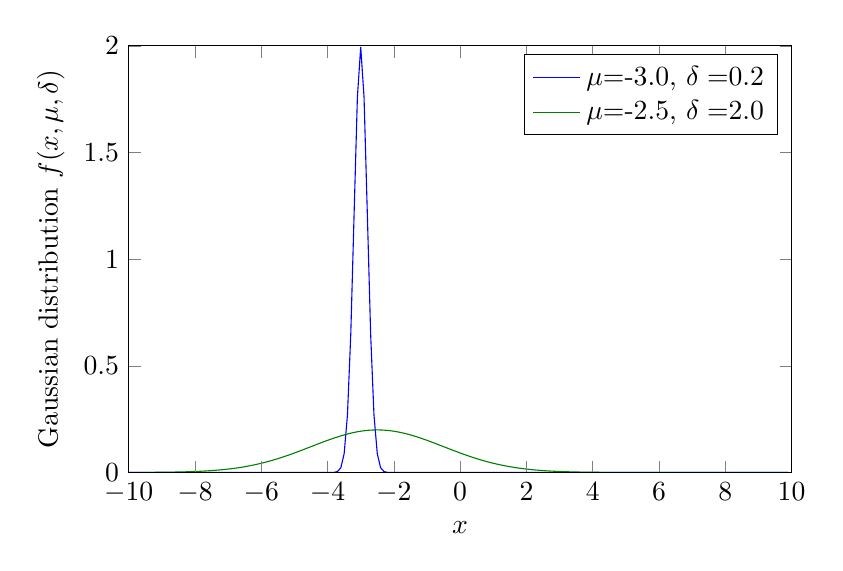
\begin{tikzpicture}

\begin{axis}[
xlabel={$x$},
ylabel={Gaussian distribution $f(x, \mu, \delta)$},
xmin=-10, xmax=10,
ymin=0, ymax=2,
axis on top,
width=10cm,
height=7cm,
legend entries={{$\mu$=-3.0, $\delta=$0.2},{$\mu$=-2.5, $\delta=$2.0}}
]
\addplot [blue]
coordinates {
(-10,1.97019813856824e-266)
(-9.9,6.92431039168968e-259)
(-9.8,1.89526320004643e-251)
(-9.7,4.04007020693576e-244)
(-9.6,6.70709833674642e-237)
(-9.5,8.67175131803119e-230)
(-9.4,8.7318312837919e-223)
(-9.3,6.8474715403965e-216)
(-9.2,4.1819758029268e-209)
(-9.1,1.98911171364038e-202)
(-9,7.36823067438939e-196)
(-8.9,2.12565917676281e-189)
(-8.8,4.77584727097171e-183)
(-8.7,8.35667682564565e-177)
(-8.6,1.13878873936762e-170)
(-8.50000000000001,1.20859028930895e-164)
(-8.40000000000001,9.98944629583458e-159)
(-8.30000000000001,6.43028337035209e-153)
(-8.20000000000001,3.22362998569636e-147)
(-8.10000000000001,1.2585968525957e-141)
(-8.00000000000001,3.82696486820643e-136)
(-7.90000000000001,9.0625139677499e-131)
(-7.80000000000001,1.6713572208958e-125)
(-7.70000000000001,2.40058039295126e-120)
(-7.60000000000001,2.68528018250785e-115)
(-7.50000000000001,2.33931840862276e-110)
(-7.40000000000001,1.5871407764111e-105)
(-7.30000000000001,8.38625261426362e-101)
(-7.20000000000001,3.45101471006018e-96)
(-7.10000000000001,1.10599219010415e-91)
(-7.00000000000001,2.76047418107706e-87)
(-6.90000000000001,5.36588917033568e-83)
(-6.80000000000001,8.1231801838595e-79)
(-6.70000000000001,9.57716245834961e-75)
(-6.60000000000001,8.79374771296627e-71)
(-6.50000000000001,6.28836191438436e-67)
(-6.40000000000001,3.50209106715551e-63)
(-6.30000000000001,1.51895084939332e-59)
(-6.20000000000001,5.13081536395412e-56)
(-6.10000000000001,1.34975651229287e-52)
(-6.00000000000001,2.76535477491934e-49)
(-5.90000000000001,4.4123774872929e-46)
(-5.80000000000001,5.48303279693925e-43)
(-5.70000000000001,5.30634406957073e-40)
(-5.60000000000001,3.99941387849937e-37)
(-5.50000000000002,2.34759767898527e-34)
(-5.40000000000002,1.07319186783049e-31)
(-5.30000000000002,3.82082770579002e-29)
(-5.20000000000002,1.05940962675369e-26)
(-5.10000000000002,2.28768779525834e-24)
(-5.00000000000002,3.84729931334982e-22)
(-4.90000000000002,5.03896769714571e-20)
(-4.80000000000002,5.13988678583022e-18)
(-4.70000000000002,4.08311781583153e-16)
(-4.60000000000002,2.52613554176653e-14)
(-4.50000000000002,1.21716026651362e-12)
(-4.40000000000002,4.56736020417913e-11)
(-4.30000000000002,1.33477830738055e-09)
(-4.20000000000002,3.03794142490978e-08)
(-4.10000000000002,5.38488002126855e-07)
(-4.00000000000002,7.43359757366754e-06)
(-3.90000000000002,7.99187055344886e-05)
(-3.80000000000002,0.000669151128824133)
(-3.70000000000002,0.0043634134752271)
(-3.60000000000002,0.0221592420596825)
(-3.50000000000002,0.0876415024678174)
(-3.40000000000002,0.269954832565877)
(-3.30000000000002,0.647587978329343)
(-3.20000000000002,1.20985362259557)
(-3.10000000000002,1.76032663382139)
(-3.00000000000002,1.99471140200716)
(-2.90000000000002,1.76032663382161)
(-2.80000000000002,1.20985362259587)
(-2.70000000000002,0.647587978329585)
(-2.60000000000002,0.269954832566011)
(-2.50000000000003,0.0876415024678719)
(-2.40000000000003,0.022159242059699)
(-2.30000000000003,0.0043634134752309)
(-2.20000000000003,0.000669151128824798)
(-2.10000000000003,7.99187055345781e-05)
(-2.00000000000003,7.43359757367678e-06)
(-1.90000000000003,5.38488002127591e-07)
(-1.80000000000003,3.03794142491431e-08)
(-1.70000000000003,1.33477830738271e-09)
(-1.60000000000003,4.56736020418708e-11)
(-1.50000000000003,1.21716026651589e-12)
(-1.40000000000003,2.52613554177154e-14)
(-1.30000000000003,4.08311781584017e-16)
(-1.20000000000003,5.13988678584173e-18)
(-1.10000000000003,5.0389676971576e-20)
(-1.00000000000003,3.84729931335939e-22)
(-0.900000000000031,2.2876877952643e-24)
(-0.800000000000031,1.0594096267566e-26)
(-0.700000000000031,3.82082770580088e-29)
(-0.600000000000032,1.0731918678337e-31)
(-0.500000000000032,2.34759767899258e-34)
(-0.400000000000032,3.99941387851233e-37)
(-0.300000000000033,5.30634406958852e-40)
(-0.200000000000033,5.48303279695834e-43)
(-0.100000000000033,4.41237748730876e-46)
(-3.37507799486048e-14,2.76535477492964e-49)
(0.0999999999999659,1.34975651229807e-52)
(0.199999999999966,5.13081536397454e-56)
(0.299999999999965,1.51895084939958e-59)
(0.399999999999965,3.50209106717044e-63)
(0.499999999999965,6.2883619144117e-67)
(0.599999999999964,8.79374771300551e-71)
(0.699999999999964,9.5771624583937e-75)
(0.799999999999964,8.12318018389805e-79)
(0.899999999999963,5.36588917036191e-83)
(0.999999999999963,2.76047418109079e-87)
(1.09999999999996,1.10599219010981e-91)
(1.19999999999996,3.45101471007813e-96)
(1.29999999999996,8.38625261430866e-101)
(1.39999999999996,1.58714077641976e-105)
(1.49999999999996,2.33931840863586e-110)
(1.59999999999996,2.68528018252312e-115)
(1.69999999999996,2.40058039296531e-120)
(1.79999999999996,1.67135722090568e-125)
(1.89999999999996,9.06251396780502e-131)
(1.99999999999996,3.82696486823036e-136)
(2.09999999999996,1.25859685260371e-141)
(2.19999999999996,3.22362998571743e-147)
(2.29999999999996,6.43028337039449e-153)
(2.39999999999996,9.98944629590159e-159)
(2.49999999999996,1.20859028931719e-164)
(2.59999999999996,1.13878873937558e-170)
(2.69999999999996,8.35667682570503e-177)
(2.79999999999996,4.77584727100618e-183)
(2.89999999999996,2.12565917677827e-189)
(2.99999999999996,7.36823067444425e-196)
(3.09999999999996,1.98911171365531e-202)
(3.19999999999996,4.18197580295913e-209)
(3.29999999999996,6.84747154045022e-216)
(3.39999999999996,8.73183128386139e-223)
(3.49999999999995,8.67175131810119e-230)
(3.59999999999995,6.70709833680132e-237)
(3.69999999999995,4.04007020696975e-244)
(3.79999999999995,1.89526320006238e-251)
(3.89999999999995,6.92431039174951e-259)
(3.99999999999995,1.97019813858548e-266)
(4.09999999999995,4.36585855034996e-274)
(4.19999999999995,7.53452358817136e-282)
(4.29999999999995,1.01267085811531e-289)
(4.39999999999995,1.06000327577243e-297)
(4.49999999999995,8.64116866150501e-306)
(4.59999999999995,5.48610526046892e-314)
(4.69999999999995,2.76676761671098e-322)
(4.79999999999995,0)
(4.89999999999995,0)
(4.99999999999995,0)
(5.09999999999995,0)
(5.19999999999995,0)
(5.29999999999995,0)
(5.39999999999995,0)
(5.49999999999995,0)
(5.59999999999995,0)
(5.69999999999995,0)
(5.79999999999995,0)
(5.89999999999995,0)
(5.99999999999995,0)
(6.09999999999995,0)
(6.19999999999995,0)
(6.29999999999994,0)
(6.39999999999995,0)
(6.49999999999995,0)
(6.59999999999994,0)
(6.69999999999994,0)
(6.79999999999994,0)
(6.89999999999995,0)
(6.99999999999994,0)
(7.09999999999994,0)
(7.19999999999994,0)
(7.29999999999994,0)
(7.39999999999994,0)
(7.49999999999994,0)
(7.59999999999994,0)
(7.69999999999994,0)
(7.79999999999994,0)
(7.89999999999994,0)
(7.99999999999994,0)
(8.09999999999994,0)
(8.19999999999994,0)
(8.29999999999994,0)
(8.39999999999994,0)
(8.49999999999994,0)
(8.59999999999994,0)
(8.69999999999994,0)
(8.79999999999994,0)
(8.89999999999994,0)
(8.99999999999994,0)
(9.09999999999993,0)
(9.19999999999994,0)
(9.29999999999994,0)
(9.39999999999993,0)
(9.49999999999993,0)
(9.59999999999993,0)
(9.69999999999994,0)
(9.79999999999993,0)
(9.89999999999993,0)

};
\addplot [green!50.0!black]
coordinates {
(-10,0.000176297841183723)
(-9.9,0.000212390135275376)
(-9.8,0.000255232487172092)
(-9.7,0.000305950965056885)
(-9.6,0.000365832231415154)
(-9.5,0.000436341347522879)
(-9.4,0.000519140647830704)
(-9.3,0.000616109584236507)
(-9.2,0.00072936540233337)
(-9.1,0.000861284469526835)
(-9,0.00101452402864988)
(-8.9,0.00119204410073241)
(-8.8,0.00139712920743971)
(-8.7,0.00163340952809995)
(-8.6,0.00190488104911089)
(-8.50000000000001,0.00221592420596899)
(-8.40000000000001,0.00257132046152695)
(-8.30000000000001,0.0029762662098879)
(-8.20000000000001,0.00343638334530696)
(-8.10000000000001,0.00395772579148995)
(-8.00000000000001,0.00454678125079548)
(-7.90000000000001,0.00521046740721124)
(-7.80000000000001,0.00595612180380253)
(-7.70000000000001,0.00679148461684274)
(-7.60000000000001,0.0077246735671975)
(-7.50000000000001,0.00876415024678417)
(-7.40000000000001,0.00991867719589755)
(-7.30000000000001,0.0111972651474213)
(-7.20000000000001,0.0126091099575971)
(-7.10000000000001,0.0141635188708004)
(-7.00000000000001,0.0158698259178335)
(-6.90000000000001,0.0177372964231155)
(-6.80000000000001,0.0197750207946849)
(-6.70000000000001,0.0219917979902133)
(-6.60000000000001,0.0243960092895911)
(-6.50000000000001,0.0269954832565937)
(-6.40000000000001,0.0297973530344077)
(-6.30000000000001,0.0328079073873379)
(-6.20000000000001,0.0360324371681085)
(-6.10000000000001,0.0394750791504466)
(-6.00000000000001,0.0431386594132552)
(-5.90000000000001,0.0470245386884429)
(-5.80000000000001,0.0511324622819884)
(-5.70000000000001,0.0554604173397271)
(-5.60000000000001,0.0600045003484921)
(-5.50000000000002,0.0647587978329451)
(-5.40000000000002,0.0697152832226793)
(-5.30000000000002,0.0748637328178716)
(-5.20000000000002,0.0801916636709589)
(-5.10000000000002,0.0856842960239027)
(-5.00000000000002,0.0913245426945099)
(-4.90000000000002,0.0970930274916054)
(-4.80000000000002,0.102968134359986)
(-4.70000000000002,0.108926088516274)
(-4.60000000000002,0.114941070342115)
(-4.50000000000002,0.120985362259571)
(-4.40000000000002,0.127029528234593)
(-4.30000000000002,0.133042624949376)
(-4.20000000000002,0.138992443065497)
(-4.10000000000002,0.14484577638074)
(-4.00000000000002,0.150568716077401)
(-3.90000000000002,0.156126966683379)
(-3.80000000000002,0.161486179833956)
(-3.70000000000002,0.166612301445899)
(-3.60000000000002,0.171471927509691)
(-3.50000000000002,0.176032663382149)
(-3.40000000000002,0.180263481230823)
(-3.30000000000002,0.184135070151661)
(-3.20000000000002,0.187620173458468)
(-3.10000000000002,0.190693907730261)
(-3.00000000000002,0.193334058401424)
(-2.90000000000002,0.195521346987727)
(-2.80000000000002,0.197239665453944)
(-2.70000000000002,0.198476273738506)
(-2.60000000000002,0.199221957047382)
(-2.50000000000003,0.199471140200716)
(-2.40000000000003,0.199221957047382)
(-2.30000000000003,0.198476273738506)
(-2.20000000000003,0.197239665453945)
(-2.10000000000003,0.195521346987728)
(-2.00000000000003,0.193334058401425)
(-1.90000000000003,0.190693907730263)
(-1.80000000000003,0.18762017345847)
(-1.70000000000003,0.184135070151663)
(-1.60000000000003,0.180263481230825)
(-1.50000000000003,0.176032663382151)
(-1.40000000000003,0.171471927509693)
(-1.30000000000003,0.166612301445901)
(-1.20000000000003,0.161486179833959)
(-1.10000000000003,0.156126966683382)
(-1.00000000000003,0.150568716077404)
(-0.900000000000031,0.144845776380743)
(-0.800000000000031,0.1389924430655)
(-0.700000000000031,0.133042624949379)
(-0.600000000000032,0.127029528234597)
(-0.500000000000032,0.120985362259574)
(-0.400000000000032,0.114941070342119)
(-0.300000000000033,0.108926088516277)
(-0.200000000000033,0.102968134359989)
(-0.100000000000033,0.0970930274916085)
(-3.37507799486048e-14,0.091324542694513)
(0.0999999999999659,0.0856842960239057)
(0.199999999999966,0.0801916636709618)
(0.299999999999965,0.0748637328178744)
(0.399999999999965,0.069715283222682)
(0.499999999999965,0.0647587978329477)
(0.599999999999964,0.0600045003484946)
(0.699999999999964,0.0554604173397295)
(0.799999999999964,0.0511324622819906)
(0.899999999999963,0.047024538688445)
(0.999999999999963,0.0431386594132572)
(1.09999999999996,0.0394750791504485)
(1.19999999999996,0.0360324371681103)
(1.29999999999996,0.0328079073873395)
(1.39999999999996,0.0297973530344092)
(1.49999999999996,0.0269954832565951)
(1.59999999999996,0.0243960092895924)
(1.69999999999996,0.0219917979902146)
(1.79999999999996,0.019775020794686)
(1.89999999999996,0.0177372964231165)
(1.99999999999996,0.0158698259178345)
(2.09999999999996,0.0141635188708013)
(2.19999999999996,0.0126091099575978)
(2.29999999999996,0.011197265147422)
(2.39999999999996,0.0099186771958982)
(2.49999999999996,0.00876415024678476)
(2.59999999999996,0.00772467356719803)
(2.69999999999996,0.00679148461684321)
(2.79999999999996,0.00595612180380295)
(2.89999999999996,0.00521046740721162)
(2.99999999999996,0.00454678125079582)
(3.09999999999996,0.00395772579149024)
(3.19999999999996,0.00343638334530722)
(3.29999999999996,0.00297626620988813)
(3.39999999999996,0.00257132046152715)
(3.49999999999995,0.00221592420596916)
(3.59999999999995,0.00190488104911104)
(3.69999999999995,0.00163340952810008)
(3.79999999999995,0.00139712920743983)
(3.89999999999995,0.00119204410073252)
(3.99999999999995,0.00101452402864997)
(4.09999999999995,0.000861284469526911)
(4.19999999999995,0.000729365402333435)
(4.29999999999995,0.000616109584236563)
(4.39999999999995,0.000519140647830751)
(4.49999999999995,0.000436341347522919)
(4.59999999999995,0.000365832231415189)
(4.69999999999995,0.000305950965056915)
(4.79999999999995,0.000255232487172117)
(4.89999999999995,0.000212390135275397)
(4.99999999999995,0.00017629784118374)
(5.09999999999995,0.000145973462895745)
(5.19999999999995,0.000120563290113009)
(5.29999999999995,9.93277356963968e-05)
(5.39999999999995,8.16282043831298e-05)
(5.49999999999995,6.691511288245e-05)
(5.59999999999995,5.47170217199064e-05)
(5.69999999999995,4.46308285885715e-05)
(5.79999999999995,3.63129651511305e-05)
(5.89999999999995,2.94715338782734e-05)
(5.99999999999995,2.38593182706054e-05)
(6.09999999999995,1.92675983710459e-05)
(6.19999999999995,1.5520703528927e-05)
(6.29999999999994,1.24712356450284e-05)
(6.39999999999995,9.99589835346271e-06)
(6.49999999999995,7.99187055345376e-06)
(6.59999999999994,6.37366619091758e-06)
(6.69999999999994,5.07042603274408e-06)
(6.79999999999994,4.02359122824671e-06)
(6.89999999999995,3.18491258943399e-06)
(6.99999999999994,2.51475364429658e-06)
(7.09999999999994,1.98064954551633e-06)
(7.19999999999994,1.5560877895747e-06)
(7.29999999999994,1.21948037294686e-06)
(7.39999999999994,9.53300451561551e-07)
(7.49999999999994,7.43359757367268e-07)
(7.59999999999994,5.78205951789982e-07)
(7.69999999999994,4.48621758119236e-07)
(7.79999999999994,3.47210117692824e-07)
(7.89999999999994,2.68051767234926e-07)
(7.99999999999994,2.06423549431534e-07)
(8.09999999999994,1.58567460835825e-07)
(8.19999999999994,1.21501927054047e-07)
(8.29999999999994,9.28680922277815e-08)
(8.39999999999994,7.08050356508185e-08)
(8.49999999999994,5.38488002127259e-08)
(8.59999999999994,4.08509518927236e-08)
(8.69999999999994,3.09131025008351e-08)
(8.79999999999994,2.33344339879757e-08)
(8.89999999999994,1.75697754741055e-08)
(8.99999999999994,1.31962160178554e-08)
(9.09999999999993,9.88659820312434e-09)
(9.19999999999994,7.3885397932415e-09)
(9.29999999999994,5.50788181234225e-09)
(9.39999999999993,4.09566920174043e-09)
(9.49999999999993,3.03794142491229e-09)
(9.59999999999993,2.24775091550709e-09)
(9.69999999999994,1.65894212177399e-09)
(9.79999999999993,1.22131741340379e-09)
(9.89999999999993,8.96891953982244e-10)

};
\path [draw=black, fill opacity=0] (axis cs:13,2)--(axis cs:13,2);

\path [draw=black, fill opacity=0] (axis cs:10,13)--(axis cs:10,13);

\path [draw=black, fill opacity=0] (axis cs:13,0)--(axis cs:13,0);

\path [draw=black, fill opacity=0] (axis cs:-10,13)--(axis cs:-10,13);

\end{axis}

\end{tikzpicture}
\end{center}
\caption{Visualization of two Gaussian distributions}
\label{fig:gaussians}
\end{figure}

%\begin{figure}[tbh]
%\begin{center}
%	\includegraphics[width=0.65\textwidth]{twogaussian.png}
%\end{center}
%\caption{Visualization of two Gaussian distributions}
%\label{fig:gaussians}
%\end{figure}

To prune hypothesis models, the Mahalanobis distance is calculated between each pair of the models. If the Mahalanobis distance is under certain threshold, the two models are considered to be close to each other, and the one with lower weight will be removed. If both weights are the same, the model with higher covariance will be removed.


\subsection{Pruning by Distance to Best Model}
\label{sub:Pruning by Distance to Best Model}

As we discussed in \autoref{sec:robotpose}, the model whichever is the ``best'' is chosen to represent the robot position. To further prune hypothesis models, the models which are very close to the ``best'' model are also removed. This distance is measured simply by Euclidean distance and the threshold is set to be a small value \SI{2}{\cm}.

